\documentclass[11pt]{beamer}

\usepackage{array}    % <-- For defining new column types
\usepackage{booktabs}
\usepackage{hyperref}
\usepackage{makecell} % <-- For multi-line cells
\usepackage[default]{opensans} 
\usepackage{pgffor}
\usepackage{pdfpages}
\usepackage{palatino}  
\usepackage{tcolorbox} 
\usepackage{textcomp}
\usepackage{ulem}
\usepackage{xcolor} 
\usepackage{tcolorbox} 
\usepackage{tikz}
\usepackage{tabularx}



\usetikzlibrary{arrows.meta} 
\usetikzlibrary{decorations.pathreplacing} 
\usetikzlibrary{decorations.pathmorphing}  
\usetikzlibrary{decorations.markings}     
\usetikzlibrary{decorations.text}      

\usepackage{listings}
\lstset{
  basicstyle=\ttfamily\small,
  columns=fullflexible,
  breaklines=true,
  frame=single,
  showstringspaces=false,
  showspaces=false,
  keepspaces=true,
  tabsize=4
}


\newtcbox{\highlighttexttt}{nobeforeafter, colframe=white, colback=lightgray!30, boxrule=0pt, arc=2pt, boxsep=0pt, left=1pt, right=1pt, top=1pt, bottom=1pt}
\newcommand{\hl}[1]{\colorbox{lightgray!30}{\texttt{#1}}}
\newcommand{\blink}[2]{\href{#1}{\textcolor{blue}{\underline{#2}}}}
\newcommand{\try}[1]{Have A Try: \blink{https://github.com/FSU-COP4610-F25/in-class-code}{#1}}

\usetheme{Madrid}
\usefonttheme{default} 

\useinnertheme{circles}

\setbeamertemplate{footline}{
    \leavevmode%
    \hbox{%
        \begin{beamercolorbox}[wd=0.92\paperwidth,ht=2.5ex,dp=1ex,left]{section in head/foot}
            \hspace{0.5em}
            \insertsectionnavigationhorizontal{0.9\paperwidth}{}{}
        \end{beamercolorbox}%
        \begin{beamercolorbox}[wd=0.08\paperwidth,ht=2.5ex,dp=1ex,right]{section in head/foot}
            \insertframenumber{} / \inserttotalframenumber
            \hspace{0.2em}
        \end{beamercolorbox}%
    }%
    \vskip0pt%
}


\setbeamersize{text margin left=1em, text margin right=1em}

\setbeamertemplate{frametitle}{
    \vspace{-0.5em} 
    \begin{beamercolorbox}[wd=\paperwidth,ht=2.5ex,dp=0.75ex,left]{frametitle} 
        \usebeamerfont{frametitle}\hspace{0.72em}\insertframetitle
    \end{beamercolorbox}
    \vspace{-0.5em} 
}


\newcommand{\FSUOSMeta}{%
  \author[Xin Liu]{\small Xin Liu}%
  \institute[FSU]{\small Florida State University\\[2pt]
    \href{mailto:xliu15@fsu.edu}{xliu15@fsu.edu}}%
  \date[\today]{\small CIS 4930/5930 Future Edge Networks\\[2pt]
    \href{https://xinliulab.github.io/FSU-CIS4930-CIS5930-Future-Edge-Networks/}
         {https://xinliulab.github.io/FSU-CIS4930-CIS5930-Future-Edge-Networks/}}%
}


\title[Synchronization]{Class 1: Preparation for Learning Edge Networks} 

\subtitle{XG History and Course Tools} 

\FSUOSMeta

\begin{document}

\begin{frame}[plain]
    \titlepage
\end{frame}

\addtocounter{framenumber}{-1}


% %!TEX root = ./main.tex


\section{Outline}

\begin{frame}
    \frametitle{Outline}

We have already learned that an "executable file" is a data structure that describes the initial state of a process. Through the Funny Little Executable, we explored the compilation, linking, and loading processes involved in generating an executable file.

    \textbf{Today's Key Question:}

    \begin{itemize}
        \item As the software ecosystem evolved, the need for \textbf{"decomposing"} software and dynamic linking emerged!
    \end{itemize}


    \vspace{15pt}

    \textbf{Main Topics for Today:}

    \begin{itemize}
        \item Dynamic Linking and Loading: Principles and Implementation
        \item Security in \textbf{libc}
    \end{itemize}

\end{frame}


%!TEX root = ./main.tex

\section{Introduction}

\begin{frame}{Meet Your Instructor}
  \begin{columns}
    \column{0.4\textwidth}
      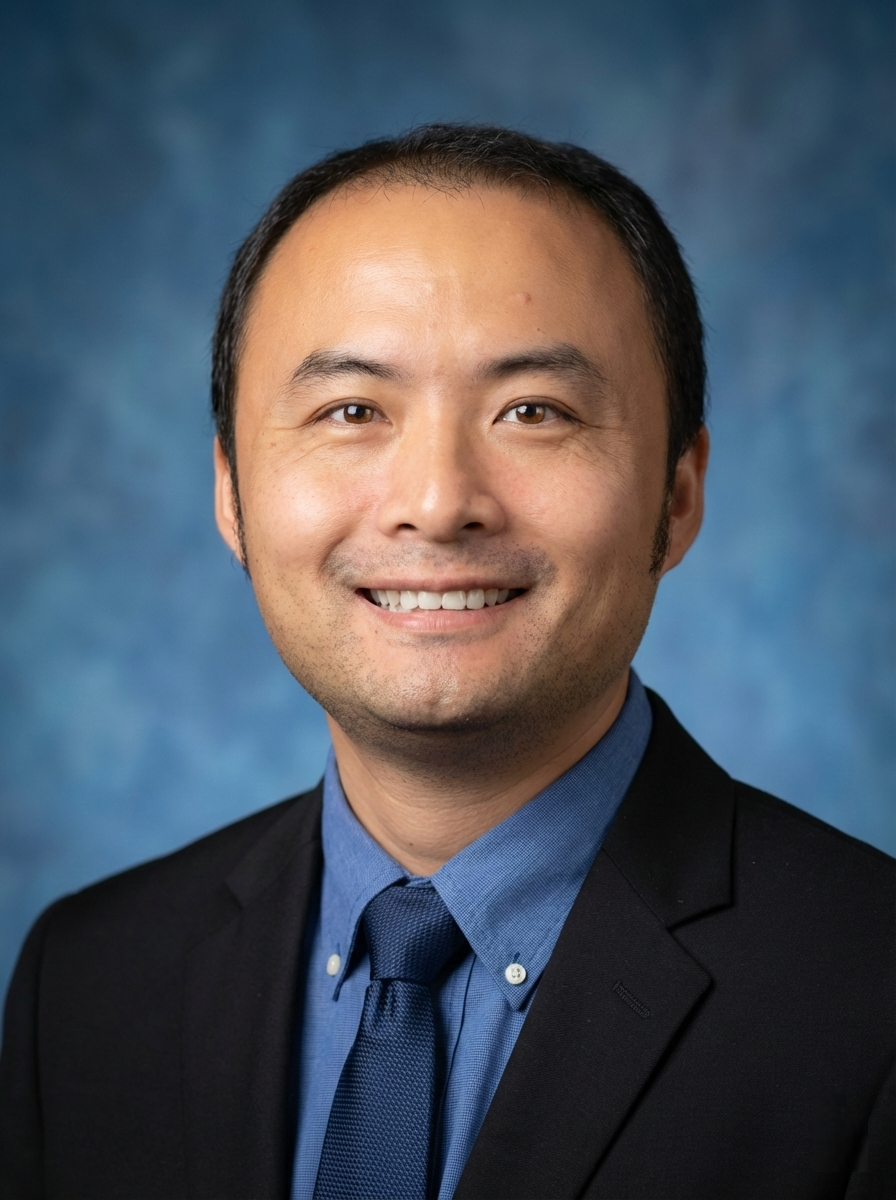
\includegraphics[width=\linewidth]{figure/headshot.png}
    \column{0.6\textwidth}
      \textbf{Xin Liu} \\
      Assistant Professor \\
      Department of Computer Science \\
      Florida State University \\
      \vspace{1em}
      Research: \\
      \textbf{AI-driven edge networks and intelligent wireless systems} \\
      \vspace{1em}
      Hobby: \textit{Not Working}\\
      \textit{Started at FSU in Fall 2024} \\
      \href{https://xinliulab.github.io/}{\textcolor{blue}{\texttt{Click here to visit my homepage}}}
  \end{columns}
\end{frame}

%!TEX root = ./main.tex

\section{XG History}

\begin{frame}{Mobile has made a leap every 10 years}
  \centering
  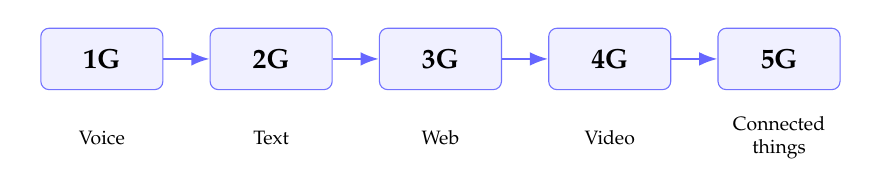
\begin{tikzpicture}[
      gen/.style={draw=blue!55, fill=blue!6, rounded corners=3pt, minimum width=1.55cm, minimum height=0.78cm, align=center, font=\bfseries},
      note/.style={align=center, font=\scriptsize, text width=1.65cm},
      >=Latex
    ]
    \node[gen] (g1) at (0,0) {1G};
    \node[gen] (g2) at (2.15,0) {2G};
    \node[gen] (g3) at (4.3,0) {3G};
    \node[gen] (g4) at (6.45,0) {4G};
    \node[gen] (g5) at (8.6,0) {5G};
    \foreach \a/\b in {g1/g2,g2/g3,g3/g4,g4/g5}
      \draw[->, thick, blue!60] (\a) -- (\b);
    \node[note] at (0,-1.0) {Voice};
    \node[note] at (2.15,-1.0) {Text};
    \node[note] at (4.3,-1.0) {Web};
    \node[note] at (6.45,-1.0) {Video};
    \node[note] at (8.6,-1.0) {Connected\\things};
  \end{tikzpicture}

  \vspace{1.0em}
  \begin{tabular}{@{}lllll@{}}
    1980s & 1990s & 2000s & 2010s & 2020s \\
  \end{tabular}

  \vspace{0.8em}
  \small
  Each generation changed what people expected a phone to do.
  The device, radio link, and battery budget moved together.
\end{frame}

\begin{frame}{Every Generation Has Its Own Sound}
  \Large
  \blink{https://www.youtube.com/watch?v=0F8AmuobbZk}{Play the Nokia ringtone memory}.

  {\tiny
  Every time I hear this tune, I remember my youth, the beautiful days, and the people who made those days bright.}

  \vspace{0.8em}
  \normalsize
  \begin{itemize}
    \item A familiar sound carried a decade of mobile culture.
    \item Ringtones made the phone personal.
    \item Polyphonic audio showed that phones had become small media devices. 
    \begin{itemize}
      \item What makes a computer powerful?
      \item Compute throughput, memory capacity, memory bandwidth, storage capacity and speed, I/O bandwidth, processing latency, energy efficiency...
    \end{itemize}
  \end{itemize}

  
\end{frame}

% \begin{frame}{Applications follow capability}
%   \begin{columns}[T]
%     \column{0.46\textwidth}
%       \Large \textbf{The phone got stronger.}
%       \vspace{0.7em}

%       \normalsize
%       \begin{itemize}
%         \item More radio throughput
%         \item More local processing
%         \item Better screens, sensors, and storage
%         \item More energy demand
%       \end{itemize}

%     \column{0.54\textwidth}
%       \Large \textbf{The default app changed.}
%       \vspace{0.7em}

%       \normalsize
%       \begin{itemize}
%         \item 1G: voice on analog cellular links
%         \item 2G: text, contact lists, and ringtones
%         \item 3G: web, email, and early video calls
%         \item 4G: maps, streaming, and short video
%         \item 5G: connected things, sensing, and edge AI
%       \end{itemize}
%   \end{columns}

%   \vspace{0.5em}
%   \small
%   A new ``G'' matters when phones, radios, and nearby computing support a new daily habit.
% \end{frame}

\begin{frame}{1G: Mobile Voice}

  \begin{columns}[T,onlytextwidth]

    \column{0.46\textwidth}
      \centering
      \begin{figure}
        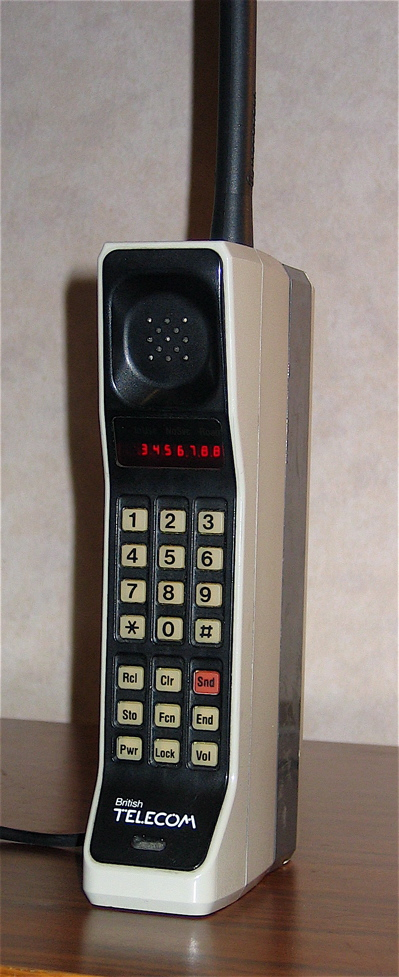
\includegraphics[height=0.64\textheight]
          {figure/xg/1g_dynatac.jpg}\\
        \vspace{0.3em}
        {\footnotesize The Motorola DynaTAC ``brick phone.''\par}
      \end{figure}

    \column{0.54\textwidth}

      \Large\textbf{The phone leaves the wall.}

      \vspace{0.8em}

      \normalsize
      \begin{itemize}
        \item Analog cellular voice
        \item Expensive devices and sparse coverage
        \item The core experience: calling from a car or the street
      \end{itemize}

  \end{columns}

\end{frame}

\begin{frame}{2G: Text goes mobile}
  \begin{columns}[T]
    \column{0.46\textwidth}
      \centering
      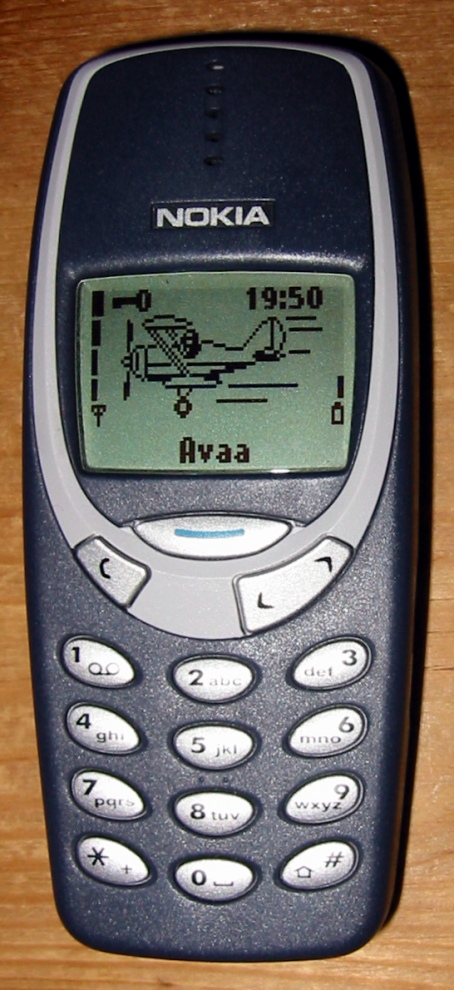
\includegraphics[height=0.64\textheight]{figure/xg/2g_nokia3310.jpg}\\
      \vspace{0.3em}
        {\footnotesize Nokia-style durable feature phones.\par}
    \column{0.54\textwidth}
      \Large \textbf{The phone becomes personal.}
      \vspace{0.8em}

      \normalsize
      \begin{itemize}
        \item Digital voice and SMS
        \item SIM cards, contacts, and prepaid plans
        \item Ringtones, Snake, and the always-on pocket device
      \end{itemize}

  \end{columns}
\end{frame}

\begin{frame}{3G: The web reaches the iPhone 4}
  \begin{columns}[T]
    \column{0.48\textwidth}
      \centering
      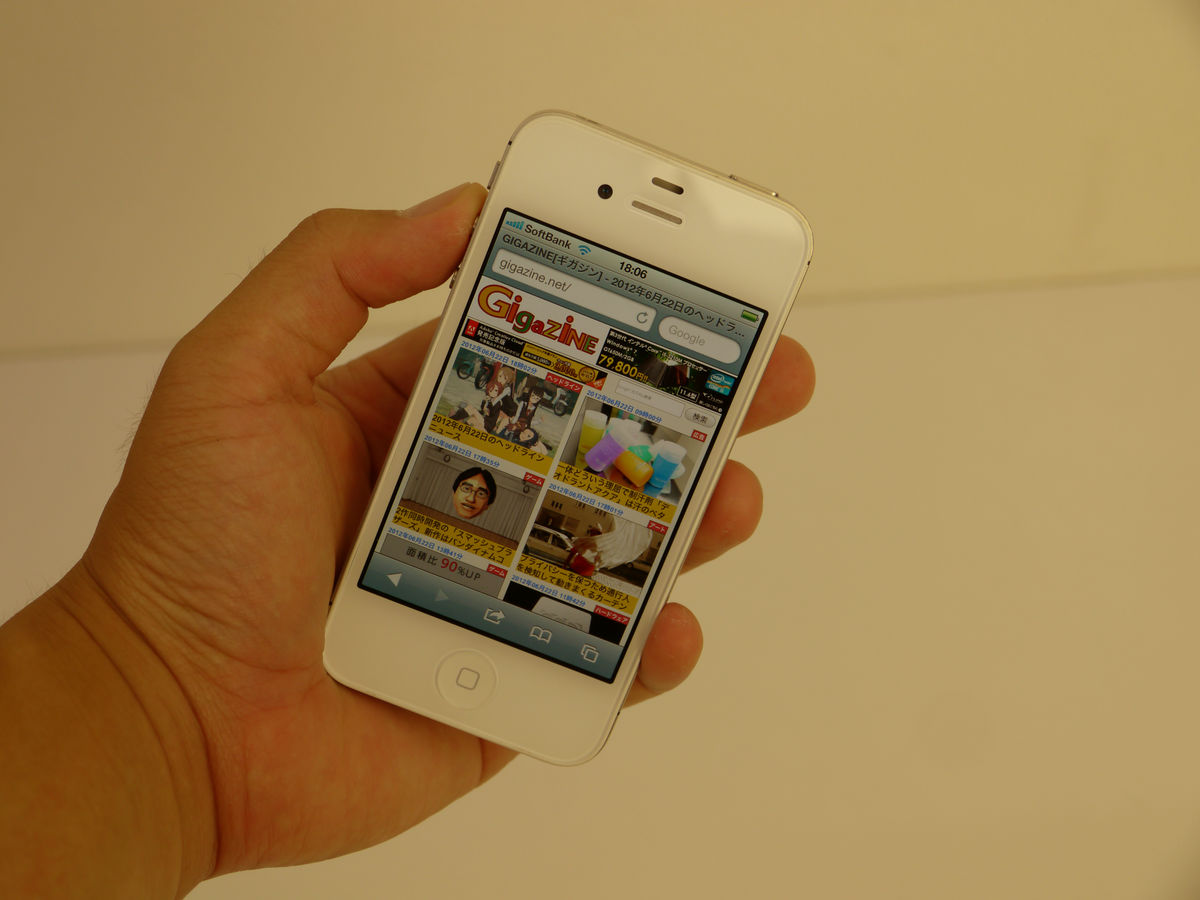
\includegraphics[width=\linewidth]{figure/xg/iphone4_white_web.jpg}\\
      \vspace{0.3em}
        {\footnotesize A white iPhone 4, a defining device of the 3G era, browsing the mobile web.\par}
    \column{0.52\textwidth}
      \Large \textbf{Data becomes the product.}
      \vspace{0.8em}

      \normalsize
      \begin{itemize}
        \item Mobile web, email, and app stores
        \item Camera phones and multimedia messages
        \item Early video calls over UMTS networks
      \end{itemize}


  \end{columns}
\end{frame}

\begin{frame}{4G: Video becomes normal}
  \begin{columns}[T]
    \column{0.50\textwidth}
      \centering
      
\includegraphics[width=\linewidth]{figure/xg/4g_tiktok_app.jpg}\\
      \vspace{0.3em}
        {\footnotesize TikTok and short-video apps.\par}
    \column{0.50\textwidth}
      \Large \textbf{The phone becomes a video network.}
      \vspace{0.8em}

      \normalsize
      \begin{itemize}
        \item LTE makes mobile broadband feel routine
        \item Streaming, ride sharing, maps, and live apps
        \item Short video turns uplink and downlink into daily traffic
      \end{itemize}

  \end{columns}
\end{frame}

\begin{frame}{5G: The network leaves the phone}
  \begin{columns}[T]
    \column{0.50\textwidth}
      \centering
      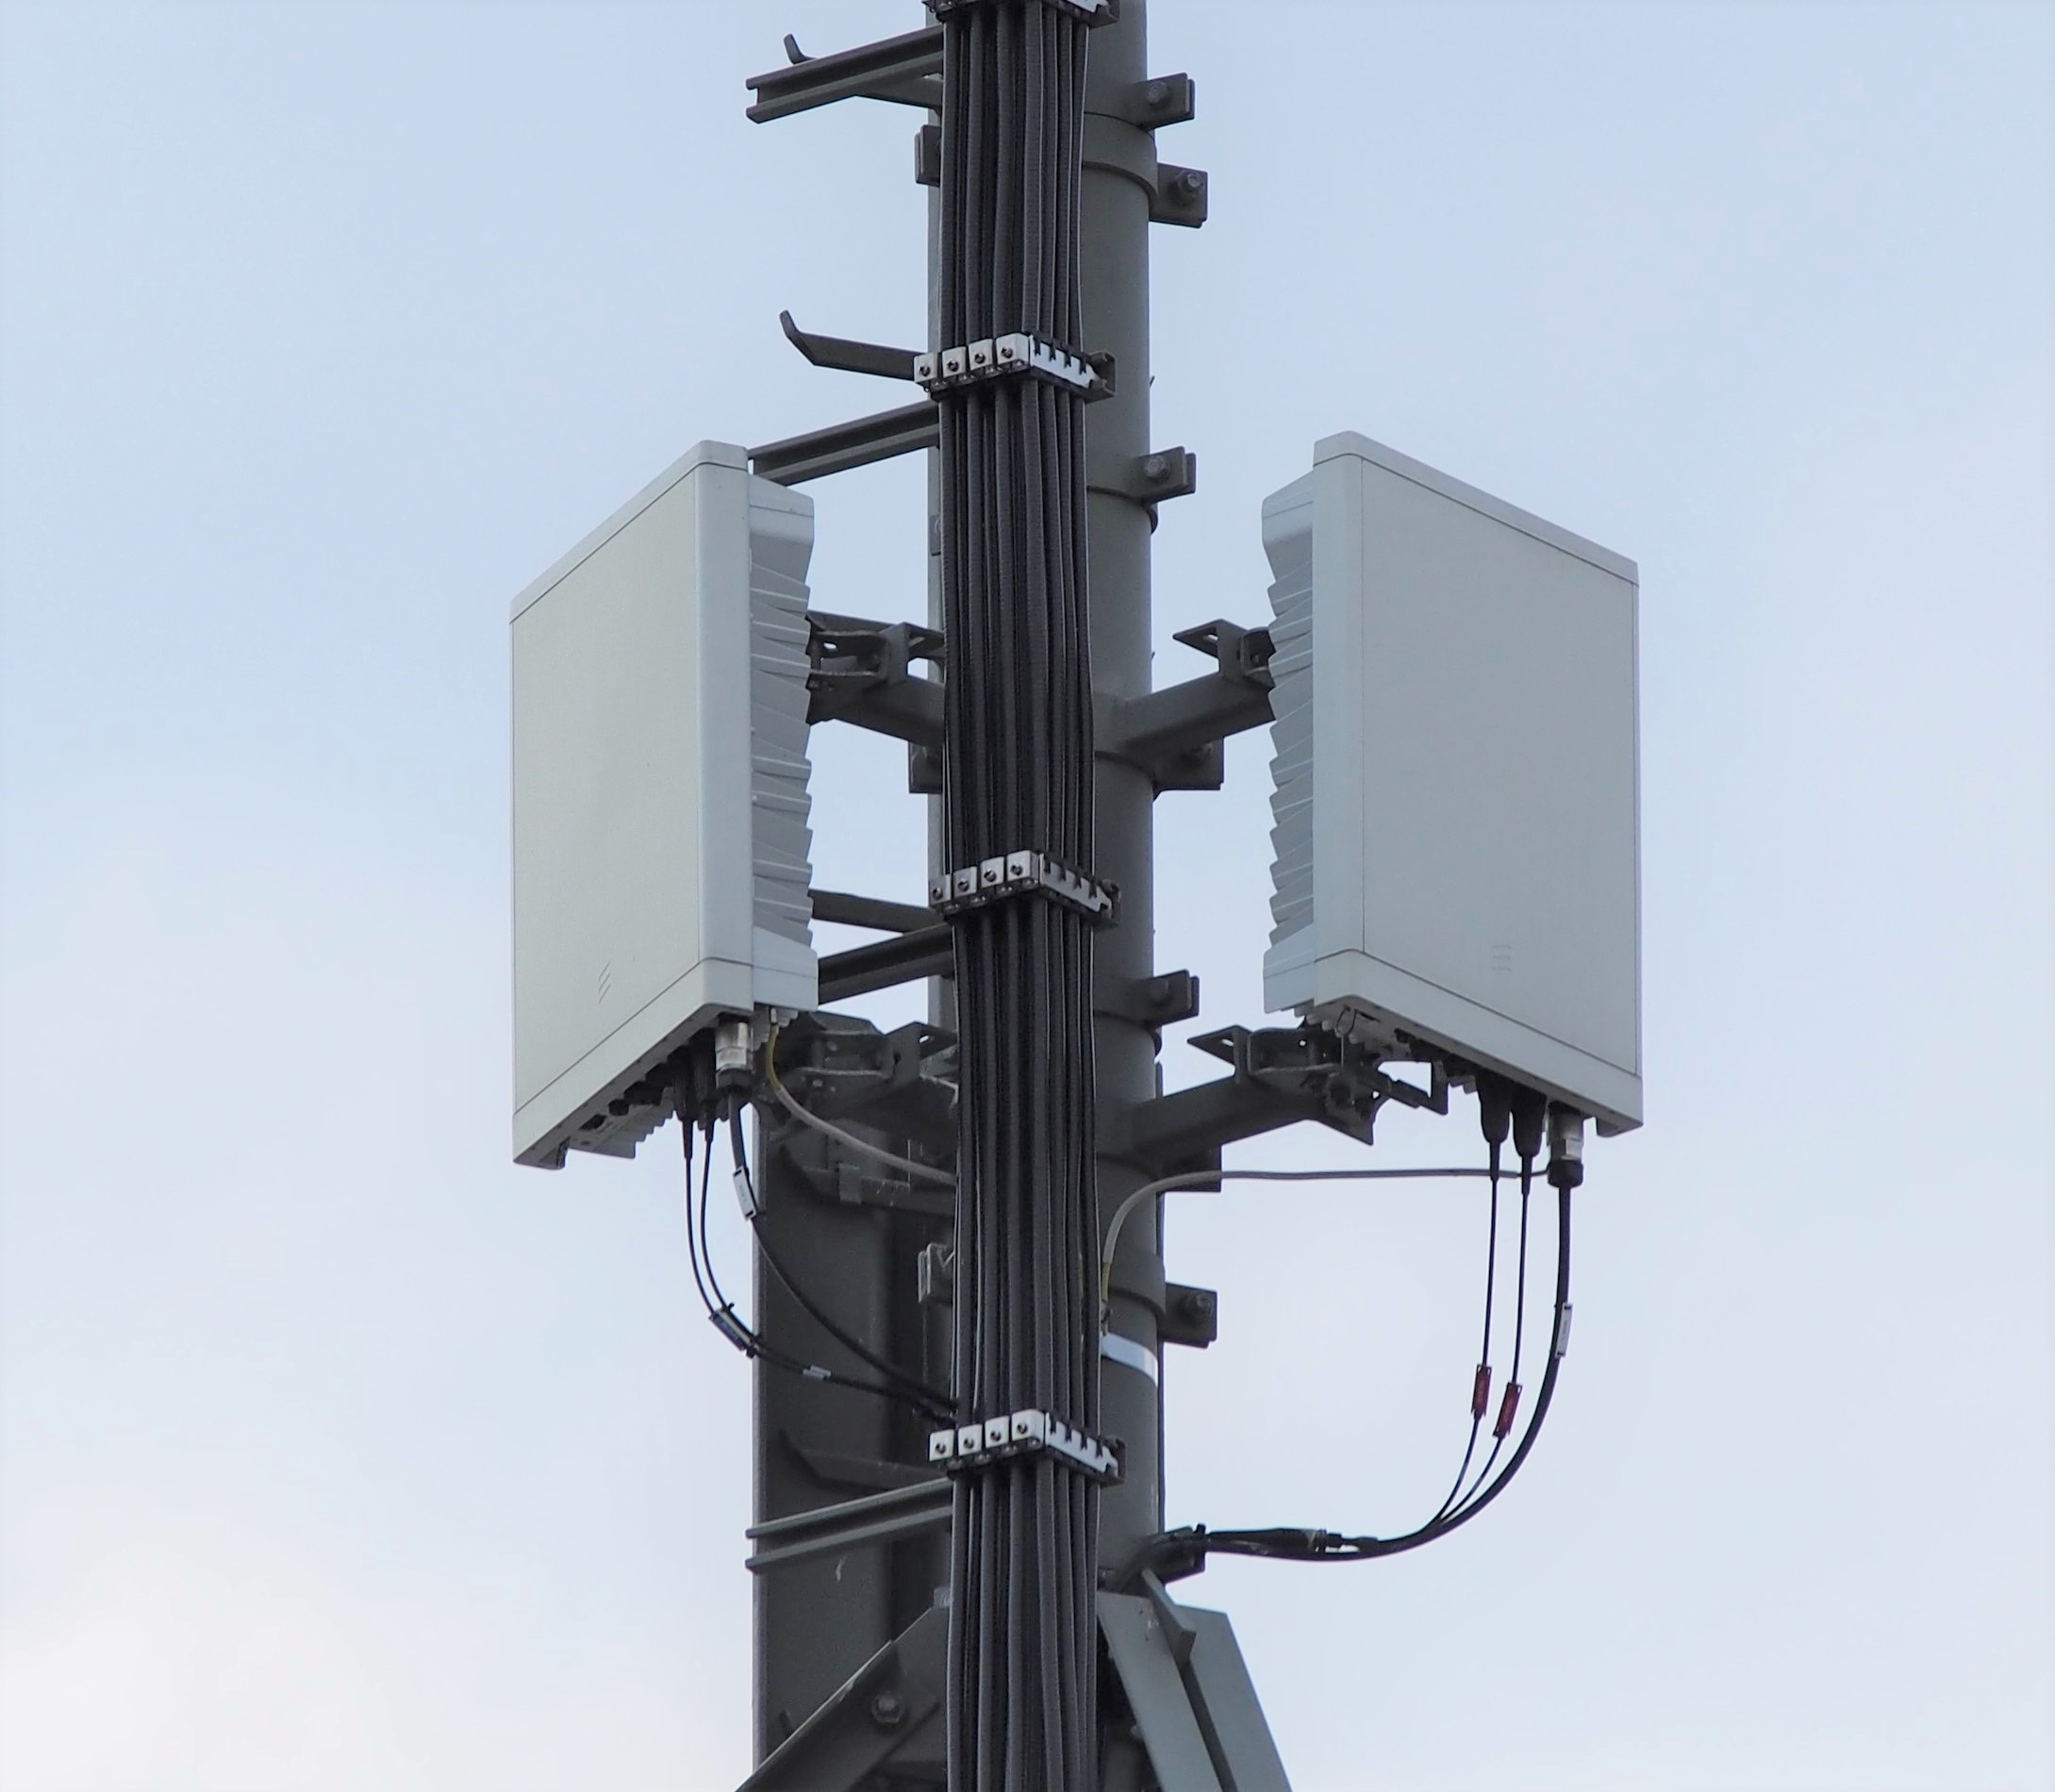
\includegraphics[width=\linewidth]{figure/xg/5g_antenna.jpg}\\
      \vspace{0.3em}
        {\footnotesize Active antenna units and dense radio sites.\par}
    \column{0.50\textwidth}
      \Large \textbf{Connectivity moves into systems.}
      \vspace{0.8em}

      \normalsize
      \begin{itemize}
        \item Enhanced mobile broadband
        \item Low-latency control and edge computing
        \item Sensing, vehicles, factories, and AI services
      \end{itemize}
     

  \end{columns}
\end{frame}

\begin{frame}{More than Technology}
  \begin{columns}[T]
    \column{0.40\textwidth}
      \centering
      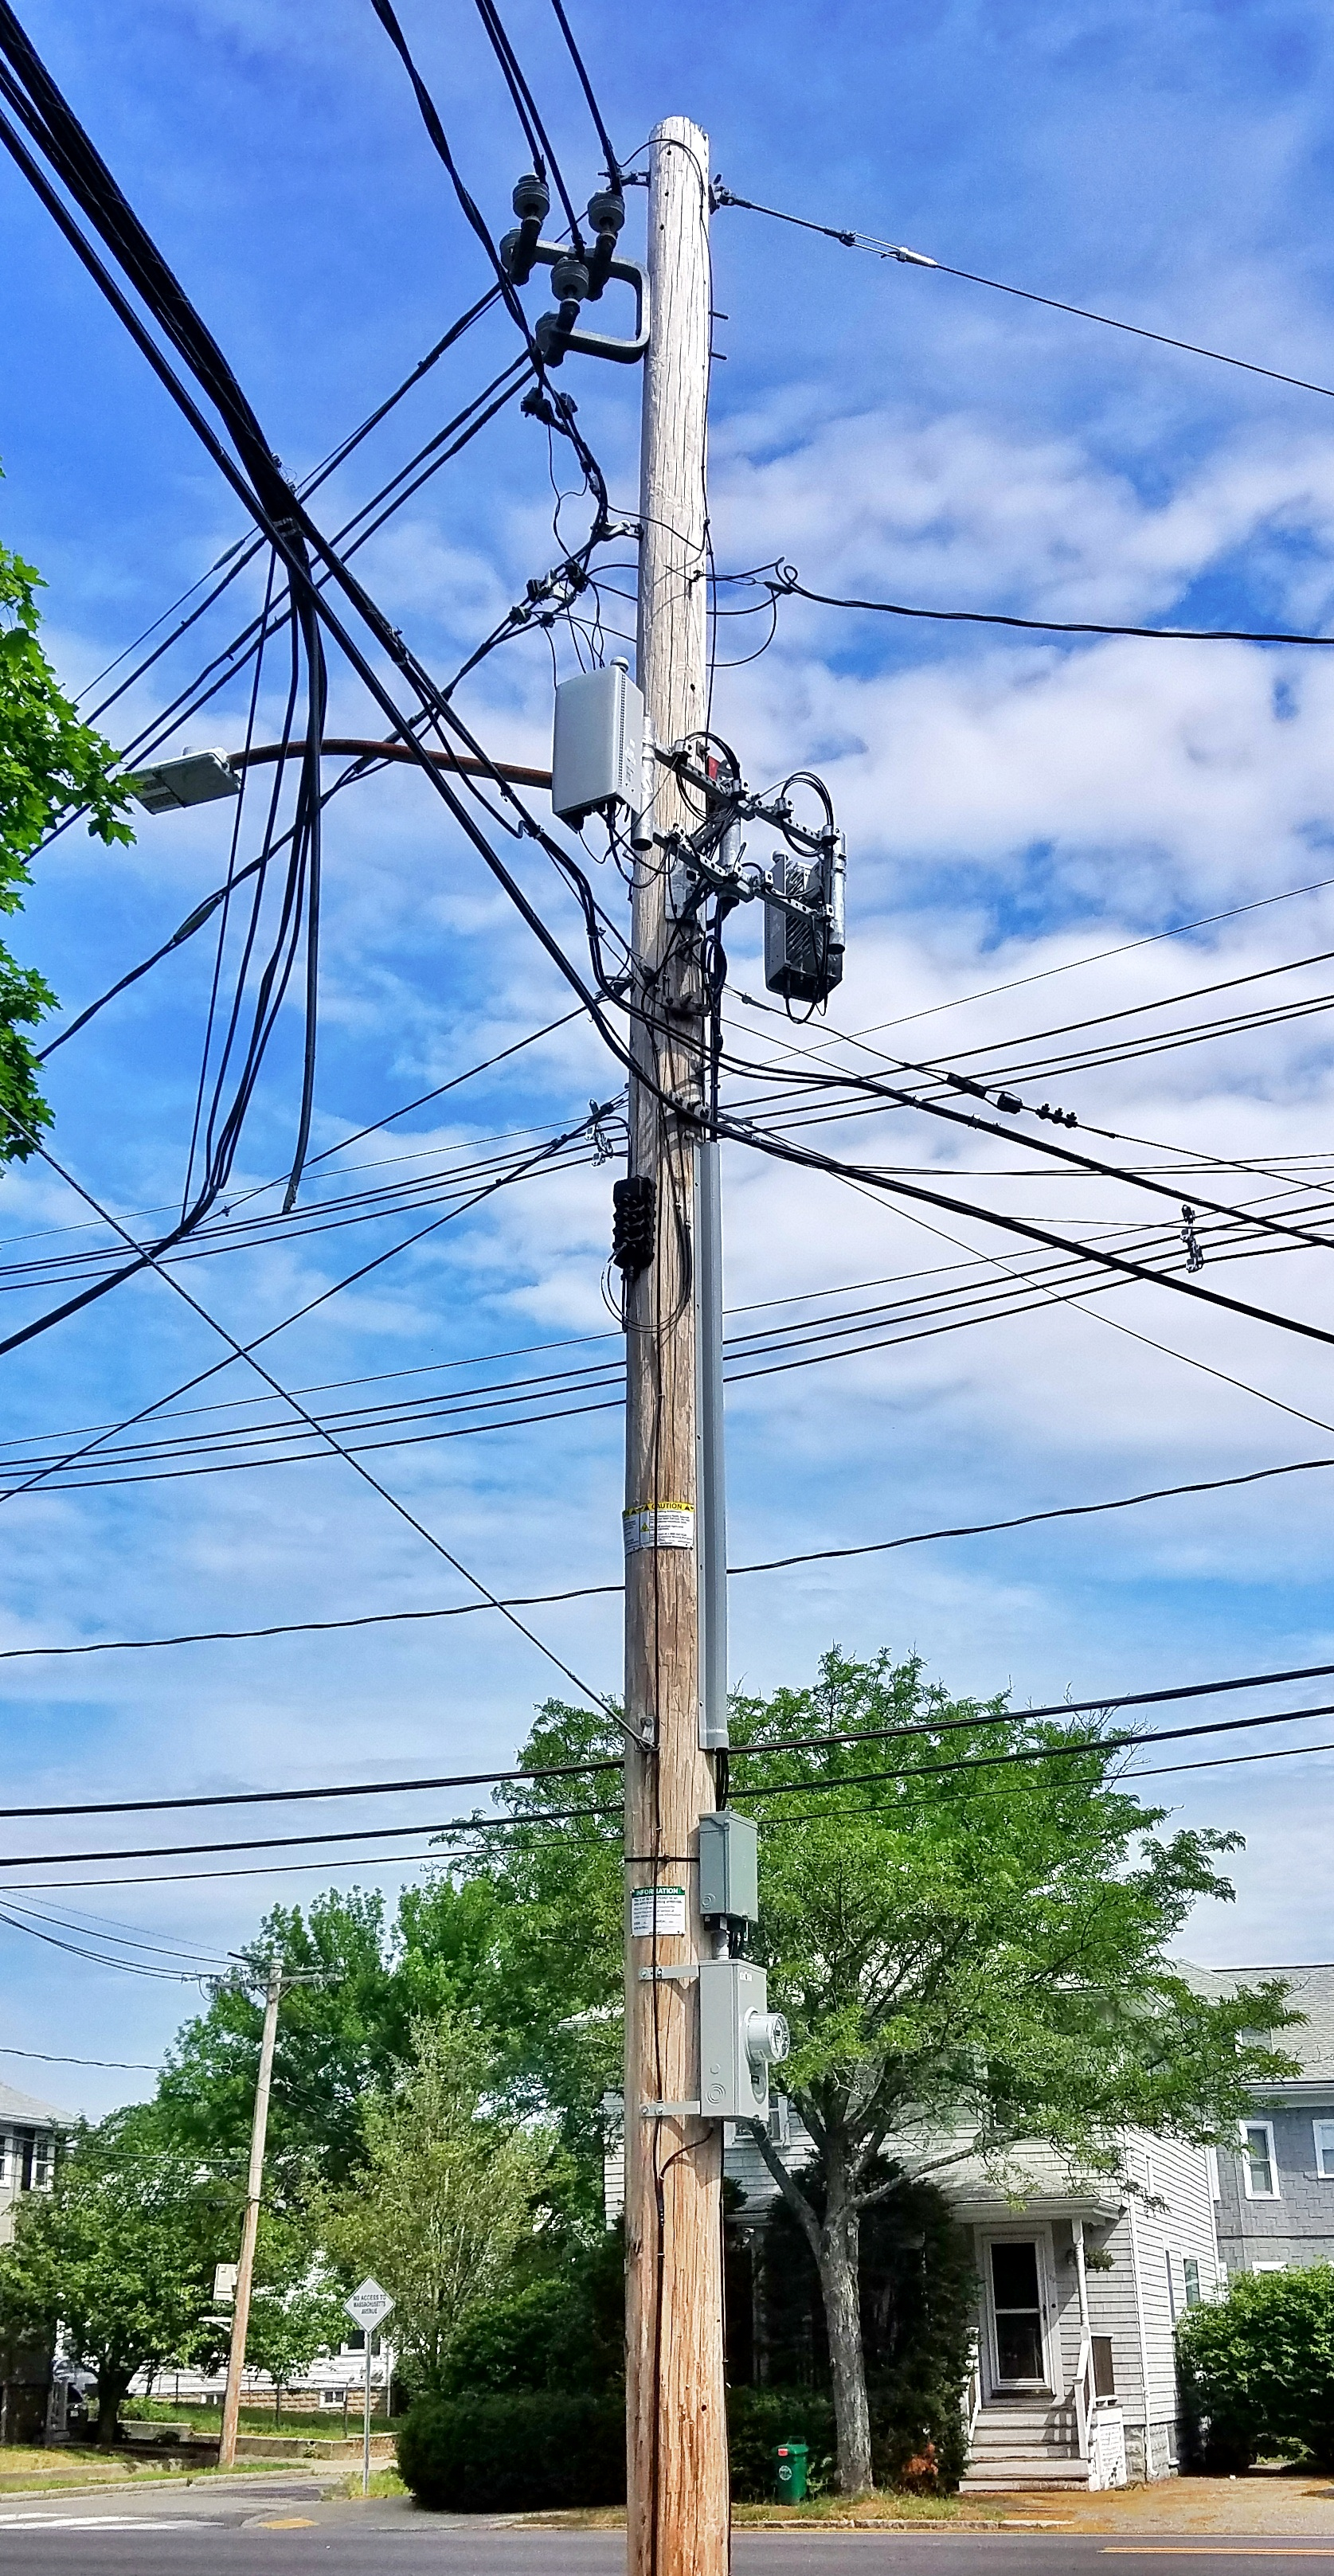
\includegraphics[height=0.7\textheight]{figure/xg/mmwave_utility_pole.jpg}\\

      \vspace{0.4em}
      {\footnotesize mmWave 5G often means dense street-level infrastructure.\par}
    \column{0.60\textwidth}
      \Large \textbf{The route matters.}
      \vspace{0.7em}

      \normalsize
      \begin{itemize}
        \item Country U had the prime mid-band spectrum tied up. Its carriers could obtain millimeter-wave spectrum more easily.
        \item Country C chose mid-band coverage first because millimeter-wave small cells cost too much at national scale.
        \item Country U fell behind in early 5G, but now returns to millimeter wave. Why? 
      \end{itemize}

  \end{columns}
\end{frame}

\begin{frame}{6G: From networks to AI systems}
  \Large
  The next ``G'' should make us ask a different question.

  \vspace{0.8em}
  \normalsize
  \begin{itemize}
    \item If every device can run or reach a large model, what should the network provide?
    \item Which tasks should stay on the device, move to nearby edge compute, or go to the cloud?
    \item What new applications appear when wireless links carry model state, sensor context, and real-time feedback?
  \end{itemize}

\end{frame}

\begin{frame}{An AI-Networking Startup: WiCi}
  \begin{columns}[T]
    \column{0.50\textwidth}
      \centering
      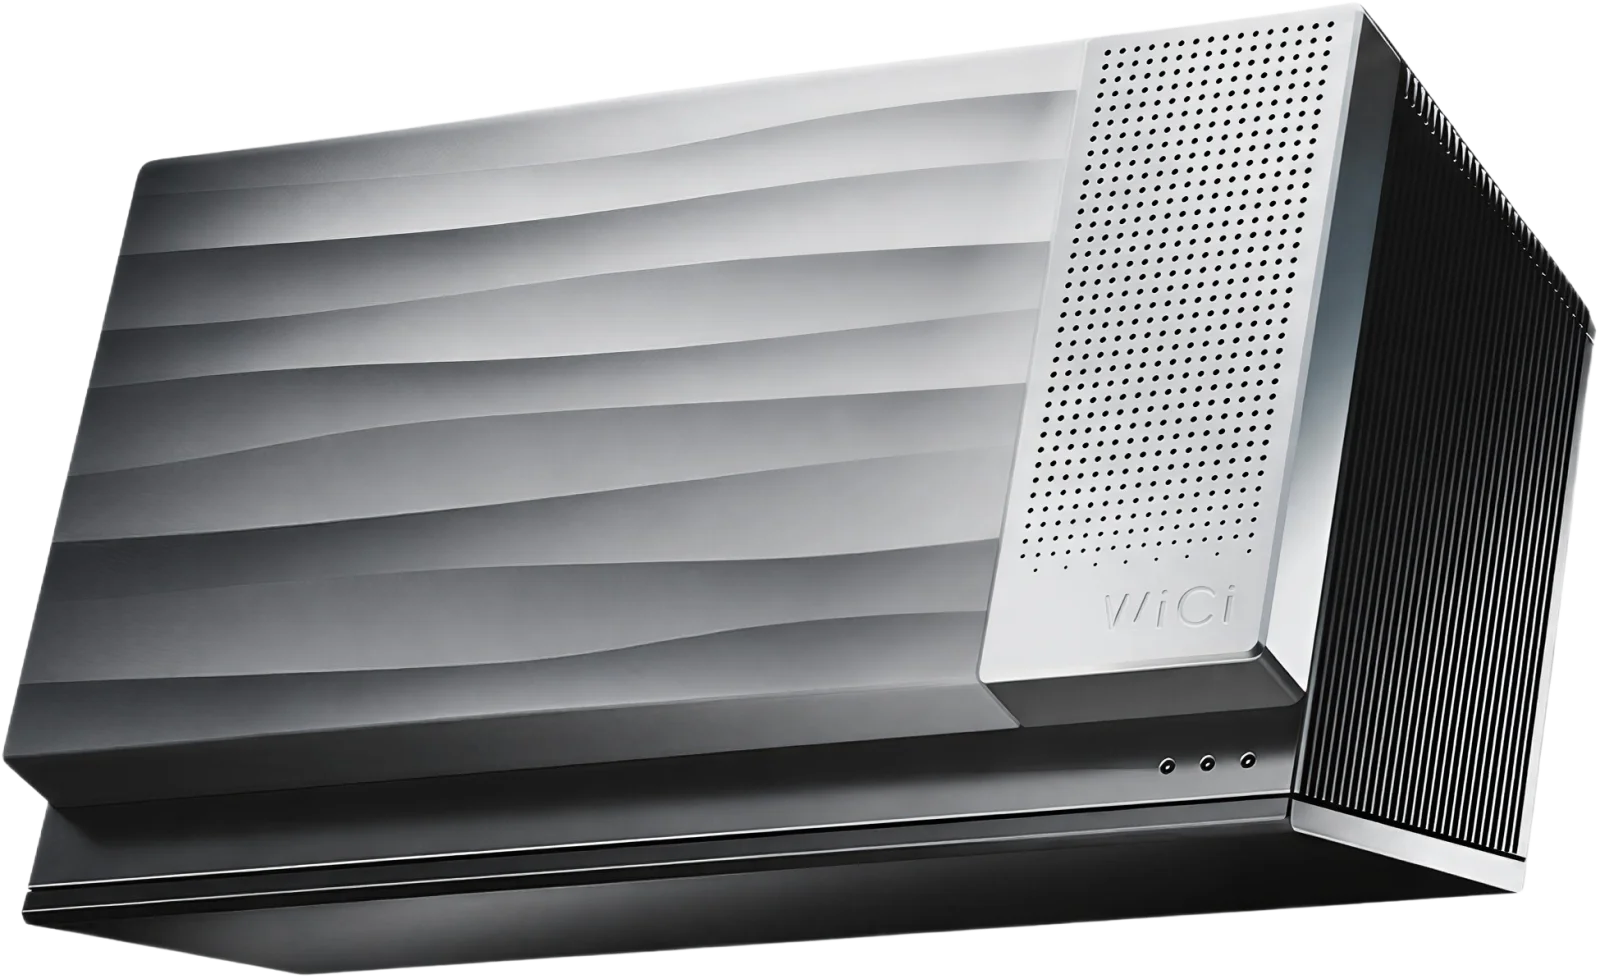
\includegraphics[width=\linewidth]{figure/xg/wici_one_product.png}\\
      \vspace{0.4em}
      \small
      \blink{https://wici.ai/wici-one}{wici.ai/wici-one}
    \column{0.50\textwidth}
      \Large \textbf{Local AI needs nearby compute.}
      \vspace{0.8em}

      \normalsize
      \begin{itemize}
        \item Phones and laptops cannot carry unlimited GPU, heat, and battery.
        \item Cloud AI adds latency, cost, privacy risk, and network dependence.
        \item WiCi One turns nearby GPU into a wireless resource.
        \item The user keeps a light device; the heavy compute stays nearby.
      \end{itemize}
  \end{columns}
\end{frame}

\begin{frame}{From 6G to XG}
  \center
  \Large
  What else could XG make possible?

\end{frame}

%!TEX root = ./main.tex
\definecolor{vscodeblue}{RGB}{0, 122, 204}
\section{Course Tools: IDE, AI, HTML, GitHub}

\begin{frame}
  \centering
  \Huge
  \textbf{Course Tools: \\IDE, AI, HTML, GitHub, }
\end{frame}


\begin{frame}
  \centering
  \Huge
  \textbf{The Best IDE in the World:}\\
  \textcolor{vscodeblue}{\textbf{Visual Studio Code}} \\[1em]

  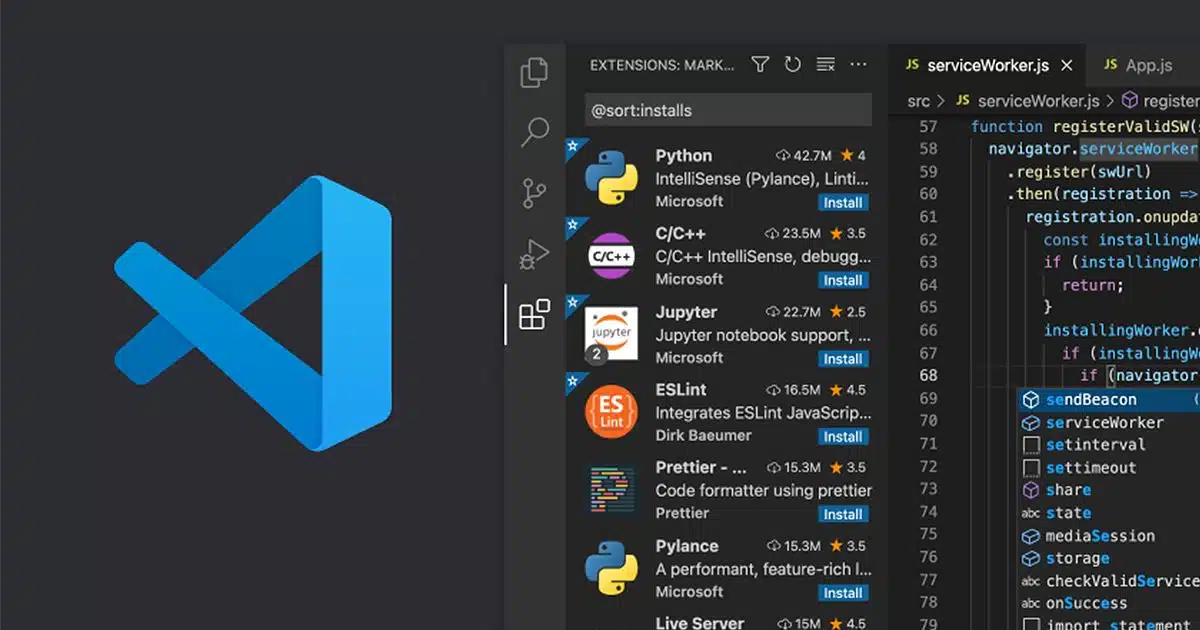
\includegraphics[width=0.92\textwidth]{figure/vs.png}
\end{frame}


\begin{frame}{Become a VS Code Master in 1 Second}
  \LARGE
  \textbf{Just remember one thing:} \\[1em]

  {\centering
  \LARGE
  \textbf{\texttt{Ctrl + Shift + P}} \\[1.5em]
  }

  \large
  This shortcut opens the Command Palette -- your gateway to: \textit{Extensions, settings, themes, terminal, and everything else.}

\end{frame}

\begin{frame}{If Ctrl + Shift + P Is Not Enough}
  \begin{columns}[T]
    \column{0.56\textwidth}
      \centering
      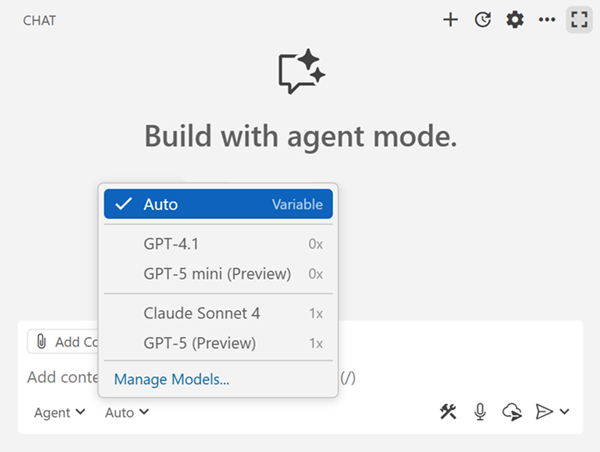
\includegraphics[width=\linewidth]{figure/vscode_agent_models.png}\\[0.35em]
      {\footnotesize VS Code agent mode can work with openAI and Claude models.\par}

    \column{0.44\textwidth}
      \Large
      \textbf{Ask an agent clearly}

      \vspace{0.8em}
      \normalsize
      \begin{itemize}
        \item Give it files, errors, screenshots, and goals
        \item Then verify: compile, run, and read the diff
      \end{itemize}
  \end{columns}
\end{frame}

%!TEX root = ./main.tex


\begin{frame}
  \centering
  \Huge
  \textbf{My View on AI}\\
  \vspace{1em}
  \large
      Can we use \textbf{ChatGPT, Claude, Gemini, Copilot, etc.} \\ to help with assignments?
\end{frame}

\begin{frame}
  \begin{columns}
    \column{0.45\textwidth}
      \Huge
      Absolutely!
    \column{0.55\textwidth}
      
\includegraphics[width=\linewidth]{figure/thanos.png}
  \end{columns}
\end{frame}



\begin{frame}{Use It!}
    \large
    \begin{itemize}
        \item You're welcome to use AI tools to brainstorm, generate code, or write explanations.
        \item You can even include notes like “This answer was inspired by ChatGPT 5.6 Sol” — that's fine.
        \item I want you to learn how to use AI productively, just like in real-world engineering.
    \end{itemize}
\end{frame}

\begin{frame}{But Outsmart It.}  

\Large    
\begin{itemize}
    \item My job is to make sure assignments are designed so that AI won’t give you perfect answers easily.
    \item Your real skill is not in copying the AI's answer— it's in understanding, adapting, and improving what AI gives you.
\end{itemize}

\vspace{1em}

\LARGE
\centering
\textcolor{red}{\textbf{\textit{AI is welcome. Lazy copying is not.}}}

\end{frame}

% \begin{frame}{The World Has Changed (cont'd)}

% \textbf{No one can stop China now}
% \begin{itemize}
%   \item The talent pipeline has reached a breakthrough point
%   \item No industry can hold back Chinese talent anymore
% \end{itemize}

% \vspace{1em}

% \textbf{Humanity has created something entirely new}
% \begin{itemize}
%   \item After prosperity, we may have to face existential questions...
%   \item Productivity gaps between people will become extreme
%   \begin{itemize}
%     \item \textcolor{blue}{The marginal return of test-driven “merit” and learning is rapidly shrinking}
%     \item AI has started to erode the value of top-tier “human labor”
%   \end{itemize}
% \end{itemize}

% \end{frame}

% \begin{frame}{We’ve Come a Long, Hard Way}

% \textbf{Everyone begins a new chapter in college}

% \begin{quote}
% \textcolor{blue}{But the first thing that hits you is a slap in the face:}
% "I once doubted if I was even fit for computer science,
% because every childhood fantasy I had about hacking 
% was crushed in my very first semester."  
% —— \href{https://csdiy.wiki}{CS Self-Study Guide}
% \end{quote}

% \begin{quote}
% Passionate and bright students… they’ve heard of relativity, quantum mechanics…
% But after slogging through the early courses (like vector calculus and electrostatics), 
% many just give up.  
% —— \textit{The Feynman Lectures on Physics}
% \end{quote}

% \vspace{1em}

% \textbf{Where is the person who lights up the dream in us?}

% \begin{quote}
% \textit{Education is not the filling of a pail, but the lighting of a fire}  
% —— William Butler Yeats
% \end{quote}

% \end{frame}


% \begin{frame}{Dream vs Reality: When I Started Teaching OS (AD 2018)}

% \textbf{Frontend programmers reshaped the open-source ecosystem}
% \begin{itemize}
%   \item ES5: 2009, React.js: 2013, VSCode: 2015, ...
%   \item “Programming” is no longer a privilege for a few geeks
% \end{itemize}

% \vspace{1em}

% \textbf{A perfect textbook finally appeared}
% \begin{itemize}
%   \item \href{https://pages.cs.wisc.edu/~remzi/OSTEP/}{\textit{Operating Systems: Three Easy Pieces}}
% \end{itemize}

% \vspace{1em}

% \textbf{After returning from the US, I saw where the bar is}
% \begin{itemize}
%   \item At least there's hope that we can live \textcolor{blue}{as well as foreigners}!
% \end{itemize}

% \vspace{1em}

% \textcolor{blue}{\textbf{But the first thing that hits you is a slap in the face:}}  
% The department made me sit behind my advisor’s chair as a TA to observe quietly…  
% Of course, such things would never be allowed to happen to someone with top honors like me!
% \end{frame}

% \begin{frame}{Dream vs Reality: When I Started Teaching OS (AD 2018)}

% \textbf{\textcolor{blue}{Altair 8800: The Machine That Launched the PC Revolution}}

% \begin{itemize}
%   \item In 1975, Bill Gates and Paul Allen implemented a full system emulator of the Altair 8800 
%         on a PDP-10 at Harvard, and wrote the first BASIC interpreter for it
%   \item With dreams (and punched tapes) in hand, they flew to MITS to demo it — and became legends
% \end{itemize}

% \vspace{1em}

% \textbf{It took us 40 years, but we made it!}
% \begin{itemize}
%   \item Today, anyone can build a full system emulator
%   \item We now have a great set of programming labs
% \end{itemize}

% \end{frame}




%!TEX root = ./main.tex

\begin{frame}{We Use HTML for Assignment Answers}

  \begin{itemize}
    \item In the past, JSON was often treated as the standard language for LLMs, APIs, configs, and structured data exchange.
    \item JSON is still useful, but it is not always the best way to communicate in AI era.
  \end{itemize}
\Large
  For this course, submit all assignment answers as
  \textbf{HTML files}.

  \medskip

  You are expected to use AI tools to help generate your HTML submissions.

  \normalsize
  \vspace{0.5em}

  \begin{itemize}
    \item HTML is readable by people and LLMs, and it can be viewed
          immediately in a web browser.

    \item It requires no Word, LaTeX, PowerPoint, or specialized viewer.
  \end{itemize}
\end{frame}

% \begin{frame}[fragile]{What Does an HTML Answer Look Like?}
%   \large
%   \textbf{HTML is both a document and a data format.}

%   \begin{itemize}
%     \item Students can write explanations, tables, figures, code blocks, and links in one file.
%     \item In the AI era, HTML is easy for both people and agents to read, generate, check, and revise.
%   \end{itemize}

%   \begin{exampleblock}{Example HTML Answer}
% \begin{verbatim}
% <section>
%   <h2>Question 1</h2>
%   <p>My answer is ...</p>
%   <pre>
% print("hello networks")
%   </pre>
% </section>
% \end{verbatim}
%   \end{exampleblock}
% \end{frame}

%!TEX root = ./main.tex

\begin{frame}{GitHub Is Our Assignment Interface}

  \begin{itemize}
    \item \textbf{One interface:} your assignment repository is the submission point.
    \item \textbf{Work in place:} code, write, test, and revise in the repo.
    \item \textbf{Submit by pushing:} your final version lives on GitHub.
    \item \textbf{Real practice:} just like in real-world engineering work.
  \end{itemize}

  \vspace{1em}
  We may occasionally use Canvas for course logistics, grades, or simple uploads.

\end{frame}


% %!TEX root = ./main.tex


\section{5G Toolbox}


% Put these frames into your Beamer file.
\begin{frame}
  \centering
  \Huge
  \textbf{MATLAB 5G Toolbox}\\
  \vspace{0.8em}
  \Large
  Do we still need to build 5G from scratch?
\end{frame}

\begin{frame}
  \begin{columns}
    \column{0.48\textwidth}
      \Huge
      Start from a reference.\\
      \vspace{0.6em}
      \Large
      MATLAB already gives you\\
      a solid 5G NR toolbox.
    \column{0.52\textwidth}
      \centering
      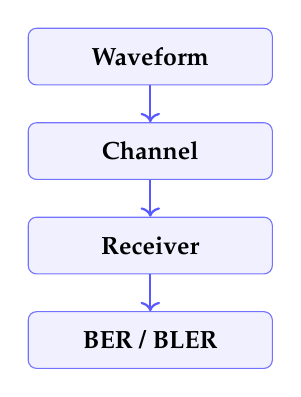
\begin{tikzpicture}[
        box/.style={draw=blue!55, fill=blue!6, rounded corners=3pt, minimum width=3.1cm, minimum height=0.72cm, align=center, font=\small\bfseries},
        arrow/.style={->, thick, blue!65}
      ]
        \node[box] (wave) at (0,1.8) {Waveform};
        \node[box] (chan) at (0,0.6) {Channel};
        \node[box] (recv) at (0,-0.6) {Receiver};
        \node[box] (metric) at (0,-1.8) {BER / BLER};
        \draw[arrow] (wave) -- (chan);
        \draw[arrow] (chan) -- (recv);
        \draw[arrow] (recv) -- (metric);
      \end{tikzpicture}
  \end{columns}
\end{frame}

\begin{frame}{What Is 5G Toolbox?}
% \Large
\begin{itemize}
  \item A MATLAB add-on to \textbf{model, simulate, analyze, and test} 5G communications systems.
  \item Built-in workflows for:
  \begin{itemize}
    \item \textbf{Waveform generation}
    \item \textbf{Link-level simulation}
    \item \textbf{Golden reference design verification}
    \item \textbf{System-level simulation}
  \end{itemize}
  \item \blink{https://www.mathworks.com/products/5g.html}{More details here}
\end{itemize}

\end{frame}

\begin{frame}{Waveforms in Minutes}
% \Large
\begin{itemize}
  \item Generate uplink and downlink waveforms with:
  \begin{itemize}
    \item \textbf{subcarrier spacing}, \textbf{bandwidth parts}, \textbf{frame numerology}
  \end{itemize}
  \item Wireless Waveform Generator app:
  \begin{itemize}
    \item \textbf{NR Test Models (NR-TM)}
    \item \textbf{Downlink Fixed Reference Channels (FRC)}
    \item For \textbf{FR1} and \textbf{FR2}
  \end{itemize}
\end{itemize}
\end{frame}

\begin{frame}{Channels and Signals You Will See in Real 5G}

\begin{itemize}
  \item Physical channels:
  \begin{itemize}
    \item Uplink/downlink shared channels
    \item Control and broadcast channels
  \end{itemize}
  \item Synchronization and reference signals:
  \begin{itemize}
    \item PSS, SSS
    \item DM-RS (demodulation, timing, sync)
    \item Phase tracking, CSI-related reference signals
    \item SRS (sounding reference signal)
    \item PRACH (random access)
  \end{itemize}
\end{itemize}
\end{frame}

\begin{frame}{Link-Level Simulation: The Classic Pipeline}
\begin{itemize}
  \item End-to-end link simulation:
  \begin{itemize}
    \item transmitter $\rightarrow$ channel $\rightarrow$ receiver
  \end{itemize}
  \item Standard channel models:
  \begin{itemize}
    \item \textbf{CDL} and \textbf{TDL} channel models
  \end{itemize}
  \item Metrics you can compute:
  \begin{itemize}
    \item BER, BLER, throughput
  \end{itemize}
  \item Receiver building blocks:
  \begin{itemize}
    \item channel/timing estimation, synchronization, equalization
  \end{itemize}
\end{itemize}
\end{frame}

\begin{frame}{Coding and Procedures Are Included}
\begin{itemize}
  \item Channel coding components:
  \begin{itemize}
    \item \textbf{LDPC} and \textbf{Polar} coding subcomponents
  \end{itemize}
  \item Initial access procedures:
  \begin{itemize}
    \item cell search and selection
    \item decode \textbf{MIB} and \textbf{SIB1}
    \item construct SS bursts and sync using DM-RS
  \end{itemize}
\end{itemize}
\end{frame}

\begin{frame}{System-Level Simulation: Multi-Node, Scheduling}
\begin{itemize}
  \item Multi-node simulations at the system level
  \item Example: \textbf{PUSCH scheduling} under different MAC strategies
  \item Great for understanding:
  \begin{itemize}
    \item RAN behaviors, resource allocation, and performance tradeoffs
  \end{itemize}
\end{itemize}
\end{frame}

\begin{frame}{The Part I Really Want You to Use}
\Large  
\centering
\textbf{It is open MATLAB source code.}\\
\vspace{0.8em}
\Large
Read it like a textbook.
\end{frame}

\begin{frame}{Why This Matters}

\begin{itemize}
  \item You can access features as \textbf{customizable MATLAB source code}.
  \item Treat it as a \textbf{golden reference} for design verification.
  \item If you dissect the implementation step by step (with the help of your GPT teacher),
  \begin{itemize}
    \item you will understand how 5G NR really works.
    \item \textcolor{red}{\textbf{you will become a 5G (6G) engineer faster}}.
  \end{itemize}

\end{itemize}

\end{frame}


%!TEX root = ./main.tex

\section{Takeaways}

\begin{frame}{Takeaways}


\begin{itemize}
  \item We are living in the \textbf{AI era}.
  \item With AI, the distance between you and “top talent” is much smaller than you think.
  \item Knowledge is no longer the bottleneck. \textbf{Curiosity is.}
  \item Your advantage is the ability to \textbf{ask good questions} and \textbf{analyze what you get}.
\end{itemize}

\vspace{0.8em}
\centering
\LARGE


\end{frame}

\end{document} 